\documentclass[10pt,twocolumn,letterpaper]{article}

\usepackage{cvpr}
\usepackage{times}
\usepackage{epsfig}
\usepackage{graphicx}
\usepackage{amsmath}
\usepackage{amssymb}
\usepackage[utf8x]{inputenc}
\renewcommand{\refname}{Bibliografia}
\usepackage{listings}
\renewcommand{\lstlistingname}{}
\renewcommand{\figurename}{Figura}


\usepackage{url}

% Include other packages here, before hyperref.

% If you comment hyperref and then uncomment it, you should delete
% egpaper.aux before re-running latex.  (Or just hit 'q' on the first latex
% run, let it finish, and you should be clear).
%\usepackage[pagebackref=true,breaklinks=true,letterpaper=true,colorlinks,bookmarks=false]{hyperref}

\cvprfinalcopy % *** Uncomment this line for the final submission

\def\cvprPaperID{****} % *** Enter the CVPR Paper ID here
\def\httilde{\mbox{\tt\raisebox{-.5ex}{\symbol{126}}}}

% Pages are numbered in submission mode, and unnumbered in camera-ready
\ifcvprfinal\pagestyle{empty}\fi
\begin{document}

%%%%%%%%% TITLE
\title{Parallel Computing Mid-Term\\DES Decryption con C, Cuda \& OpenMP}

\maketitle
\thispagestyle{empty}

%%%%%%%%% ABSTRACT
\begin{abstract}
   L'obiettivo di questo progetto è quello di decifrare una password di 8 caratteri avendo a disposizione il suo valore di hash, generato tramite algoritmo DES (Data Encryption Standard) e supponendo di conoscere il "salt" con cui è stata cifrata la password. In questa relazione verranno presentati tre approcci diversi: uno sequenziale (in C) e due paralleli (con CUDA e OpenMP).
\end{abstract}

%%%%%%%%% BODY TEXT
\section{Introduzione}
In questo progetto vogliamo confrontare i tempi di esecuzione di un \textit{attacco con dizionario} all'algoritmo di cifratura DES utilizzando tre metodologie diverse. Con l'espressione \textit{attacco con dizionario} si intende una tecnica di attacco alla sicurezza di un sistema, in cui si suppone di avere un dizionario di password in chiaro e fornendo una password cifrata, il programma dovrebbe scoprire se si trova nel dizionario, cifrando ad una ad una ogni parola per poi confrontare il risultato con l'hash della password.

\subsection{DES}
Il DES (Data Encryption Standard) è un algoritmo di cifratura basato su chiave simmetrica per cifrare e decifrare dati, risalente agli anni '70. Attualmente il DES è considerato insicuro perchè la chiave utilizzata per la cifratura è di soli 56 bit, il che lo rende facilmente vulnerabile agli attacchi. Negli ultimi anni tale algoritmo è stato sostituito dall'AES (Advanced Encryption Standard).\cite{DES} 

\subsection{Descrizione del Dataset}
Il dataset utilizzato per gli esperimenti è stato estratto da uno più grande contenente 10 milioni di password\cite{DATASET}. Con uno script Python abbiamo estratto solo le password lunghe 8 caratteri e appartenenti al set [a-zA-z0-9]. Il dizionario finale contiene quindi un milione e mezzo di password.
\subsubsection{Scelta delle Password da testare}
Per un confronto più accurato delle esecuzioni sequenziali e parallele, anziché selezionare le password casualmente dal dataset, sono state scelte 10 password uniformemente distribuite lungo il dizionario: \textit{'sirpizza', '3kingdom', 'tyleisha', 'marumari', 'giacomix', 'dbcookie', 'Yessssss', 'Mypaypa1', '6Melissa', '1Mazzola'}.\newline
Di queste dieci, per valutare lo Speedup delle versioni parallele, ne sono state selezionate soltanto tre (una all'inizio \textit{'3kingdom'}, una nel mezzo \textit{'giacomix'} e una alla fine \textit{'1Mazzola'} del dizionario).

\subsection{Specifiche Hardware}
Per questi esperimenti è stata utilizzata un'istanza \textit{EC2} di \textit{Amazon Web Services} con le seguenti specifiche:
\begin{itemize}
\item \textit{p2.xlarge} con accelerazione del calcolo
\item Processore a 2,3 GHz (base) e 2,7 GHz (turbo) Intel Xeon E5-2686 v4
\item GPU NVIDIA K80 ad alte prestazioni, ognuna con 2.496 core di elaborazione in parallelo
\item 4 CPU virtuali
\item 90 GiB di memoria CPU e 12 GiB di memoria GPU
\end{itemize} 

\section{Implementazione}
Sono state eseguite tre implementazioni, una in maniera sequenziale in linguaggio C e due in maniera parallela rispettivamente con CUDA e OpenMP.\newline
L'algoritmo DES non è stato implementato ma è stata usata la funzione \textit{crypt} per il C e \textit{crypt\_r} per OpenMP, definite entrambe nell'header \textit{"crypt.h"}. Per quanto riguarda CUDA è stato utilizzata un'implementazione open-source del DES specifica per la piattaforma. \cite{DES-CUDA}\newline
Come \textit{"salt"}, per cifrare le password, è stata utilizzata una parola di due caratteri ("PC", Parallel Computing), in modo che \textit{crypt} e \textit{crypt\_r} usino l'algoritmo DES e non MD5, come indicato nel manuale della libreria GNU. \cite{SALT}

\subsection{Versione Sequenziale in C}
La versione sequenziale dell'algoritmo è piuttosto semplice. Dato in input il dizionario e la password cifrata da cercare, si scorre tutto il dizionario e ad ogni passo viene cifrata la parola corrente usando l'algoritmo DES. Se i due hash sono uguali il ciclo viene interrotto e la password è trovata. Si itera fino alla fine del dizionario.\newline

Per misurare il tempo di esecuzione di questa ricerca è stata usata la funzione \textit{clock} della libreria C \textit{"time.h"} che restituisce il tempo di CPU espresso in unità \textit{clock\_t} (colpi di clock). Per ottenere il risultato in secondi si divide per la costante CLOCKS\_PER\_SEC.
\newline

\begin{lstlisting}[basicstyle=\small, language=C, frame=single, caption={Esempio di ricerca sequenziale nel dizionario}, captionpos=b]
const char* password = "3kingdom";
char* enc = strdup(crypt(password, SALT));
clock_t s = clock();

while ((getline(&cur, &len, dict)) != -1) {
  char* enc = strdup(crypt(current, SALT));
  if (strcmp(enc, enc_pass) == 0) {
    // Password trovata!
    clock_t e = clock();
    float t = (float)(e-s)/CLOCKS_PER_SEC;
    break;
  }
}
\end{lstlisting}

\subsection{Versione Parallela con CUDA}
La versione parallela con CUDA prende in input il dizionario e la password cifrata da cercare. In questo caso però tutte le parole sono state convertite in \textit{uint64\_t} (interi a 64 bit) per adeguarsi alla libreria usata per la cifratura DES. \cite{DES-CUDA} Dopo aver allocato e copiato la memoria da \textit{Host} a \textit{Device}, si effettua il lancio del \textit{Kernel} con dimensione dei blocchi e dei grid variabile.
\begin{lstlisting}[basicstyle=\scriptsize, language=C, frame=single, caption={Esempio di lancio del kernel in CUDA},captionpos=b]
// Organizzazione blocchi e grid
dim3 blockDim(blockSize);
dim3 gridDim(DICTIONARY_SIZE/blockDim.x + 1);

// Lancio kernel
kernel<<<gridDim, blockDim>>>(device_dictionary);
\end{lstlisting}

Se la password è stata trovata si misura il tempo di esecuzione utilizzando la funzione \textit{clock} della libreria C \textit{"time.h"} che restituisce il tempo di CPU espresso in unità \textit{clock\_t} (colpi di clock). Per ottenere il risultato in secondi si divide per la costante CLOCKS\_PER\_SEC.\newline
Il \textit{"salt"} e la password cifrata da cercare sono salvate nella \textit{Constant Memory}, dato che sono informazioni che non variano durante l'esecuzione del kernel e richiedono la sola lettura.\newline
Il dizionario di parole viene passato in input al kernel, eseguito in parallelo dai vari thread della GPU. Ogni thread controlla una sola parola in base all'indice calcolato a partire dalle sue coordinate (\textit{blockIdx.x, blockDim.x e threadIdx.x}). Viene eseguito un controllo per verificare se il thread entra nei limiti delle dimensioni del dizionario, per evitare \textit{overflow} al contorno dell'ultimo blocco.  
\newline
\begin{lstlisting}[basicstyle=\scriptsize, language=C, frame=single, caption={Esempio di kernel in CUDA},captionpos=b]
__constant__ uint64_t salt;
__constant__ uint64_t encryptedPassword;

__global__ void kernel(uint64_t *dict) {
  int idx = blockIdx.x * blockDim.x + threadIdx.x;
  if (idx < DICTIONARY_SIZE) {
    uint64_t cur_psw = dict[idx];
    uint64_t enc = full_des_encode_block(cur_psw, salt);
    if (enc == encryptedPassword) {
      // Password trovata!
      return;
    }
  }
}
\end{lstlisting}

\subsection{Versione Parallela con OpenMP}
Per la versione parallela con OpenMP è stata creata una classe \textit{"Decrypter"}, il cui costruttore prende in ingresso il nome del file relativo al dizionario e il \textit{"salt"}. Ogni parola del dizionario viene inserita in un vettore di stringhe, \textit{fullDictionary}, variabile privata della classe. All'interno di \textit{"Decrypter"} è stato dichiarato anche un metodo \textit{setPassword} che salva in una variabile privata la password cifrata tramite la funzione \textit{crypt}. Il metodo \textit{decrypt} prende in ingresso il numero di thread che utilizza nella direttiva di OpenMP \textit{\#pragma omp parallel num\_threads}.\newline
Si scorre tutto il dizionario utilizzando la direttiva \textit{\#pragma omp for} e all'interno del ciclo la parola corrente viene cifrata tramite la funzione \textit{crypt\_r}, che è la versione \textit{reentrant} di \textit{crypt}.\newline
Se la password è stata trovata, dato che in OpenMP i cicli non possono essere interrotti, è stata utilizzata una variabile booleana di tipo \textit{volatile} in modo da garantire la consistenza nella lettura del valore di tale variabile da parte di tutti i thread, e per fare in modo che, avendo trovato la parola, tutti i thread successivi non eseguano alcuna istruzione.\newline
Il tempo di esecuzione è stato misurato utilizzando il metodo \textit{now()} della classe \textit{steady\_clock} della libreria \textit{chrono}.
\clearpage
\begin{lstlisting}[basicstyle=\scriptsize, language=C++, frame=single, caption={Esempio di ricerca in parallelo con OpenMP},captionpos=b]
double Decrypter::decrypt(int threads) {

  volatile bool found = false;
  auto start = chrono::steady_clock::now();

#pragma omp parallel num_threads(threads)
    {
  struct crypt_data data;
  data.initialized = 0;

#pragma omp for
  for (int i = 0; i < dict.size(); i++) {
    if (found) continue;
    char *current = crypt_r(dict[i], salt, &data);
    if (strcmp(current, encrypted) == 0) {
       // Password trovata!
       found = true;
    }
  }
    }

  if (found) {
    auto end = chrono::steady_clock::now();
    std::chrono::duration<double> s = end - start;
    return s.count();
  } else {
    return 0;
  }
}
\end{lstlisting}

\section{Esperimenti \& Risultati}
Per ogni esperimento sono state eseguite 5 iterazioni per avere un misura più accurata dei vari risultati.\newline
Tutti i grafici presentati di seguito sono stati generati con uno script Python utilizzando la libreria \textit{"matplotlib"}.\newline
La bontà dei tempi di esecuzione ottenuti è stata valutata tramite la metrica dello \textit{Speedup} (S), definito come il rapporto tra il tempo di esecuzione sequenziale ($t_s$) e il tempo di esecuzione parallelo ($t_p$): $S = \frac{t_s}{t_p}$.

\subsection{Valutazione dello Speedup con CUDA}
Date tre parole posizionate rispettivamente una all'inizio (\textit{"3kingdom"}), una in mezzo (\textit{"giacomix"}) e una alla fine (\textit{"6Melissa"}) del dizionario, è stato misurato lo Speedup al variare del numero di thread per blocco.\newline
In particolare sono stati usati 8, 16, 32, 64, 128, 256, 512 thread per blocco (\textit{block\_size}). Dunque il numero di blocchi per ogni grid è data dalla formula: $\frac{dictionary\_size}{block\_size}+1$, dove $dictionary\_size$ è il numero di parole presenti nel dizionario.
\begin{figure}[h]
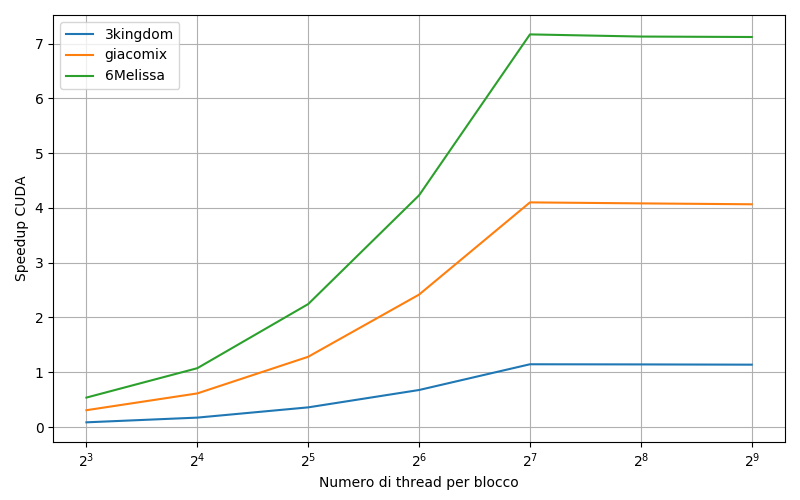
\includegraphics[width=\linewidth]{Plots/tempi_cuda.png}
\caption{Speedup in CUDA}
\end{figure}

Come si può vedere dall'immagine lo Speedup maggiore si ottiene con le parole posizionate in fondo al dizionario e il suo valore cresce all'aumentare del numero di thread per blocco, stabilizzandosi dopo 128 thread per blocco. Come era verosimile aspettarsi per parole all'inizio del dizionario risulta più efficiente la versione sequenziale ($Speedup \le 1$) soprattutto per un numero limitato di thread.

\subsection{Valutazione dello Speedup con OpenMP}
Date tre parole posizionate rispettivamente una all'inizio (\textit{"3kingdom"}), una in mezzo (\textit{"giacomix"}) e una alla fine (\textit{"6Melissa"}) del dizionario, è stato misurato lo Speedup al variare del numero di thread.\newline
In particolare sono stati usati 8, 16, 32, 64, 128, 256, 512, 1024, 2048, 4096 thread.

\begin{figure}[h]
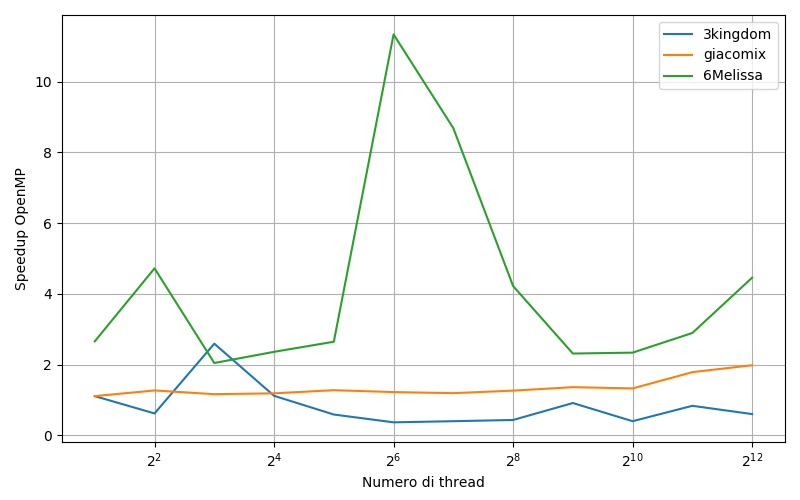
\includegraphics[width=\linewidth]{Plots/tempi_openmp.png}
\caption{Speedup in OpenMP}
\end{figure}

Come si può vedere dall'immagine lo Speedup maggiore si ottiene con le parole posizionate in fondo al dizionario, in particolare con la parola \textit{"6Melissa"} presa in esame è possibile ottenere uno Speedup maggiore di 11 con 64 thread. Questo si tratta però di un caso fortunato in quanto lo Speedup dipende dalla posizione nel \textit{chunk} di OpenMP.
Per le parole all'inizio del dizionario come ad esempio per \textit{"3kingdom"} la parallelizzazione con OpenMP risulta poco efficiente anche all'aumentare del numero di thread in confronto alla versione sequenziale (infatti $Speedup \le 1$ quasi ovunque). Questo risultato può essere attribuito all'elevato \textit{overhead} introdotto dalla gestione dei thread.
\subsection{Confronto sui Tempi di Esecuzione}
Dopo un'attenta analisi sono state scelte 10 parole uniformemente distribuite lungo il dizionario, in modo da poter confrontare direttamente i tre approcci diversi (C, CUDA e OpenMP) in alcuni casi particolari. \newline
In CUDA è stato scelto il caso con 128 thread per blocco, per OpenMP invece è stato scelto il caso con 32 thread.

\begin{figure}[h]
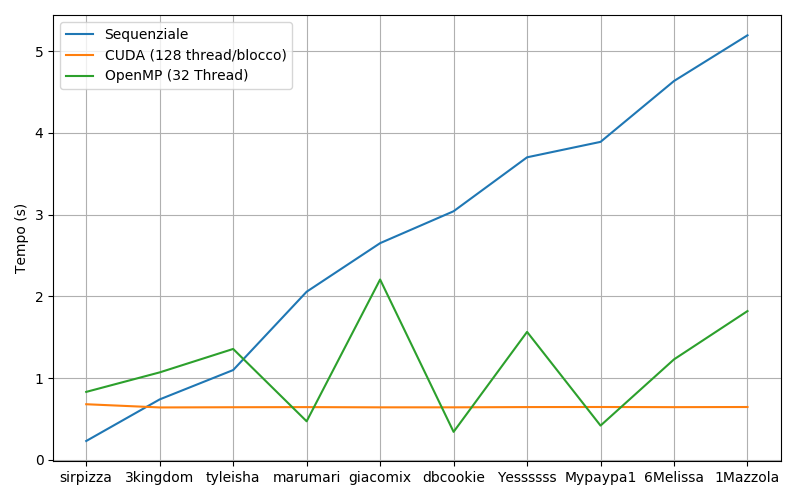
\includegraphics[width=\linewidth]{Plots/tempi.png}
\caption{Confronto tempi di esecuzione}
\end{figure}

Come si può chiaramente notare dalla figura da un certo punto in poi del dizionario ($\approx25\%$) gli approcci paralleli risultano sempre più efficienti rispetto all'approccio sequenziale.\newline
In CUDA indipendentemente dalla posizione nel dizionario della parola scelta, il tempo di esecuzione rimane costante ($\approx0.7$ secondi).
Con OpenMP il tempo di esecuzione oscilla, riuscendo ad avere in alcuni casi tempi di esecuzioni inferiori ai tempi con CUDA. Questo dipende dalla posizione della parola nel \textit{chunk} di OpenMP.
La versione sequenziale invece aumenta il suo tempo di esecuzione in maniera lineare con l'aumentare della posizione delle parole verso il fondo del dizionario. 

\section{Conclusione}
Come era possibile aspettarsi il migliore approccio per un \textit{attacco con dizionario} risulta essere quello parallelo.\newline
In quanto in entrambi i casi (CUDA \& OpenMP), aumentando il numero di thread che possono ricercare la parola desiderata nel dizionario, si ottimizza il tempo di esecuzione rispetto alla versione sequenziale (C).\newline
Dunque il problema principale delle versioni parallele potrebbe essere quello della ricerca del numero ottimale dei thread affinché si ottenga lo Speedup migliore.
Tra i due approcci paralleli OpenMP è sicuramente più facile da implementare rispetto a CUDA, in quanto la parallelizzazione avviene in maniera automatica.\newline
D'altro canto CUDA risulta più complesso da utilizzare e richiede l'impiego di una o più GPU, ma offre un tempo di esecuzione costante.


{
\bibliographystyle{unsrt}
\bibliography{bibliografia.bib}
}


\end{document}
